\begin{concept} {Nullfolgenkriterium}\\
    $\sum_{k=1}^\infty a_k~\text{konvergiert} \Rightarrow \lim_{k \to \infty} a_k = 0$ aber die Umkehrung stimmt nicht.
\end{concept}
\begin{concept} {Cauchy Kriterium}\\
    Die Reihe $\sum_{k=1}^\infty a_k$ ist genau dann konvergent, falls:\\
    $\forall \varepsilon > 0 ~\exists N \geq 1$ mit $\left|\sum_{k=n}^m a_k \right| < \varepsilon \quad \forall m \geq n \geq N$
\end{concept}
\begin{concept} {Leibniz Kriterium}\\
    Sei $\sequence$ monoton fallend, mit $a_n \geq 0~\forall n \geq 1$ und $\lim_{n \to \infty} a_n = 0$. Dann konvergiert\\
    $S \coloneqq \sum_{k = 1}^{\infty} (-1)^{k+1} a_k$
    und es gilt: $a_1 - a_2 \leq S \leq a_1$.
\end{concept}
\begin{concept} {Majorantenkriterium}\\
    Seien $a_n, b_n \geq 0$ mit $a_n \geq b_n \quad \forall n > n_0$:\\
    $\sum_{n=0}^\infty a_n$ konvergiert $\Rightarrow \sum_{n=0}^\infty b_n$ konvergiert 
\end{concept}
\begin{concept} {Minorantenkriterium}\\
    Seien $a_n, b_n \geq 0$ mit $a_n \leq b_n \quad \forall n > n_0$:\\
    $\sum_{n=0}^\infty a_n$ divergiert $\Rightarrow \sum_{n=0}^\infty b_n$ divergiert 
\end{concept}
\begin{concept} {Quotientenkriterium}\\
    Sei $\sequence$ mit $a_n \neq 0~\forall n \geq 1$ und: $q = \frac{|a_{n + 1}|}{|a_n|}$\\
    Falls:
    \begin{itemize}
        \item $q < 1$ konvergiert $\sum_{n=1}^\infty a_n$ absolut
        \item $q > 1$ divergiert $\sum_{n=1}^\infty a_n$
    \end{itemize}
    Für $\liminf a_n = 1$ keine Aussage möglich\\
    \emph{!!! für die harmonische Reihe ist dieses Kriterium nicht anwendbar/gültig !!!}
\end{concept}
\begin{concept} {Wurzelkriterium}\\
    Es sei: $q = \sqrt[n]{|a_n|}$\\
    Dann gilt:
    \begin{itemize}
        \item $q < 1 \Rightarrow \sum_{n=1}^\infty a_n$ konvergiert 
        \item $q > 1 \Rightarrow \sum_{n=1}^\infty a_n$ und $\sum_{n=1}^\infty |a_n|$ divergieren
        \item $q = 1 \Rightarrow$ keine Aussage möglich
    \end{itemize}
\end{concept}
\begin{KR}{Logarithmus abschätzen}\\
    $\log_b (n)$ kann mit $n^\alpha$ ($\alpha > 0$) abgeschätzt werden.\\
    $\ln(n) \leq \sqrt{n}$
\end{KR} 
\begin{KR}{Integral Test}\\
    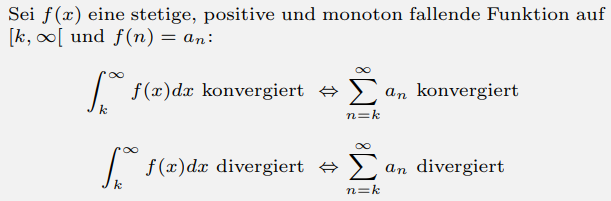
\includegraphics[scale=0.5]{Analysis1/zsf/Images/Folgen_Reihen/integraltest.png}
\end{KR}